\section{Modelagem e Implementação}

A linguagem escolhida para implementação foi Python 3(versão 3.6.0), por apresentar diversas funcionalidades de alto nível já implementadas, assim me dando a liberdade necessária para que eu pudesse focar mais nos detalhes realmente importantes da implementação. O código do trabalho pode ser encontrado em \url{https://github.com/joaofbsm/p-medians}. 

Toda a implementação foi baseada no artigo de França et al \cite{de2005max}. Esse artigo descreve um \textit{Min Max Ant System}(MMAS) modificado e adequado para resolver o problema das p-medianas com restrições de capacidades. Alguns problemas foram encontrados na descrição da implementação, presente no artigo, e esse fatores serão discutidos mais para frente. 

\subsection{Representação do mundo}

O mundo no qual o problema está inserido foi modelado com um vetor de entidades \textbf{Node}, que possuem uma posição no espaço bidimensional, uma capacidade, uma demanda e um nível de feromônios, e uma matriz de distâncias euclidiana entre os nós, onde os nós são indexados de acordo com sua posição no vetor inicialmente citado. 

\subsection{Heurística de informação}

\cite{de2005max} apresenta uma heurística de informação, baseada na densidade de clusters ao redor dos nós, a fim de melhorar a solução do sistema. Ela diz respeito à qualidade de escolha de cada nó como parte da solução, e é usada no momento de escolha das medianas. O pseudocódigo para geração do vetor com as densidades é mostrado na subseção 4.2 do artigo.

\subsection{Escolha das medianas}

A escolha das medianas é o primeiro passo do algoritmo, que, para este fim, faz o uso de um algoritmo de otimização de colônia de formigas(ACO) conhecido como \textit{Min Max Ant System}(MMAS). Esse sistema difere de um \textit{Ant System} clássico pois impõe \textit{thresholds} inferiores(min) e superiores(max) nos valores dos feromônios. Os valores mínimo($\tau_{min}$) e máximo($\tau_{max}$) são setados para 0.001 e 0.999, respectivamente, e o valor inicial para 0.5, como especificado em \cite{de2005max}. Os feromônios nessa implementação ficam nos nós, e não nas arestas como no ACO clássico.

Na seção 3.1 de \cite{de2005max} é apresentado o algoritmo para um \textit{Ant System}, no entanto um para o MMAS nunca é mostrado. O pseudocódigo seguido na implementação do MMAS é descrito no Algoritmo \ref{alg:mmas}

\medskip
\begin{lstlisting}[label=alg:mmas, caption=Pseudocódigo para o Min Max Ant System.]
	def MMAS(world, colony):
    	world.reset_pheromones(initial_pheromone)
        global_best = Solution(distance=inf)
        for i in range(n_iterations):
        	for ant in colony.ants:
            	ant.build_solution(world)
            best, worst = evaluate_solutions(world, colony)
            world.update_pheromones(decay, global_best, best, worst)
            if is_stagnated(world, max_pheromone, min_pheromone):
            	world.reset_pheromones(initial_pheromone)
            if best.distance < global_best.distance:
            	global_best = best
              
\end{lstlisting}
\medskip

Ao chamarmos \texttt{build\_solution}, utilizamos cada formiga na colônia para gerar uma solução. Uma formiga escolhe $p$ entre $n$ pontos totais para se tornarem medianas. A escolha é feita de forma probabilística e a cada iteração o nó escolhido é retirado do cálculo. A probabilidade de escolha de um nó é calculada como descrito a seguir:

\begin{figure}[H]	
  \centering
  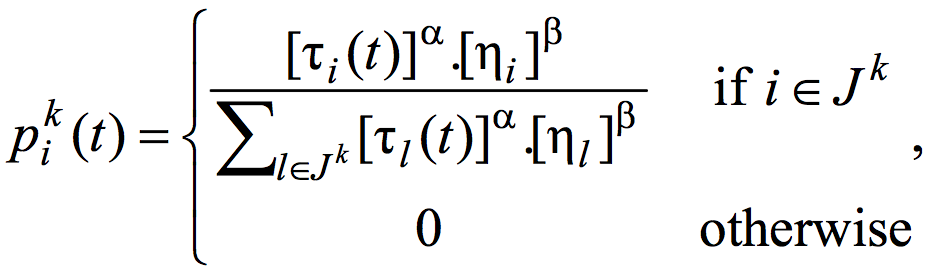
\includegraphics[width=5.3cm,keepaspectratio]{images/probabilities.png}
\end{figure}

onde $\alpha$ e $\beta$ são parâmetros definidos pelo usuário para controlar o peso da trilha de feromônios $\theta_i(t)$, com $i$ sendo o nó e $t$ a iteração corrente, e da heurística de informação $\eta_i$ no cálculo da probabilidade de escolha de um nó.

\texttt{evaluate\_solutions} avalia as soluções geradas ao atribuir os nós às medianas usando a heurística construtiva para o GAP, explorada melhor na subseção \ref{sub:gap}. As funções \texttt{update\_pheromones} e \texttt{is\_stagnated} são discutidas nas subseções \ref{sub:update-pheromone} e \ref{sub:stagnation}, respectivamente.

\subsection{Heurística para GAP} \label{sub:gap}
\textit{General Assignment Problem}(GAP) é um problema de otimização combinatória, sendo a generalização do problema de atribuição. O GAP pode ser descrito como a atribuição de um número de agentes à um número de tarefas, visando maximizar um ganho. No problema em questão ele visa minimizar a seguinte função objetivo:

\begin{figure}[H]	
  \centering
  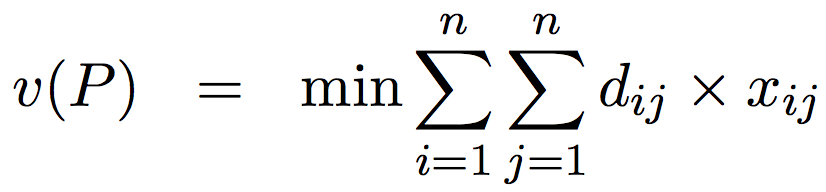
\includegraphics[width=4cm,keepaspectratio]{images/objective_function.png}
\end{figure}

onde $n$ é o número de vértices na rede, $P$ é o número de centros (medianas) a serem
localizados e $[d_{ij}] n \times n$ é uma matriz de custos (distâncias). Além disso temos uma matriz de associação entre os nós descrita como:

\begin{figure}[H]	
  \centering
  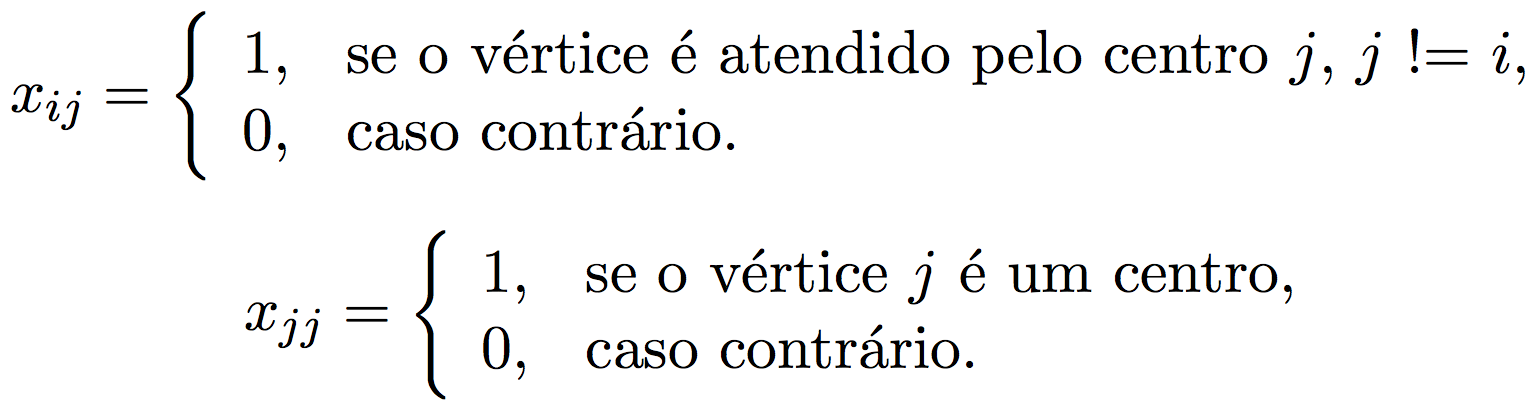
\includegraphics[width=7.5cm,keepaspectratio]{images/association.png}
\end{figure}

\cite{de2005max} apresenta uma heurística construtiva para solução do GAP na subseção 4.1, a qual foi reproduzida na Figura \ref{fig:gap}. No entanto, essa heurística não está correta, pois ela acaba gerando muitas soluções inválidas, uma vez que, com frequência, existem nós que não conseguem ser atribuídos a nenhuma mediana por problemas de excesso de capacidade. Portanto foi feita uma alteração na mesma, para que, ao ordenarmos os clientes, ao invés de usarmos a distância como fator, usamos a demanda de cada nó, em ordem decrescente. 

\begin{figure}[h]	
  \centering
  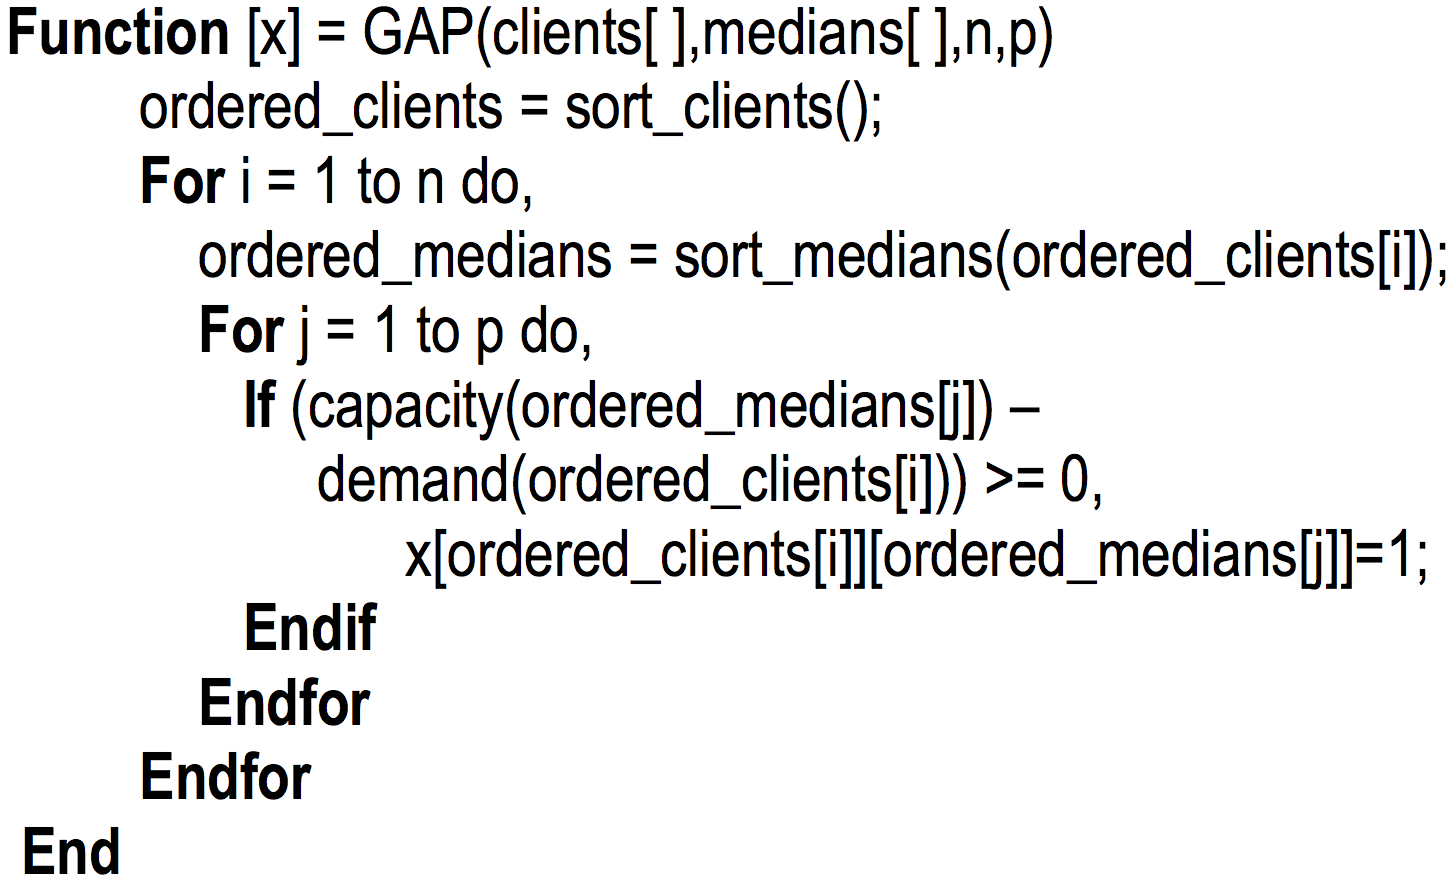
\includegraphics[width=7cm,keepaspectratio]{images/gap.png}
  \caption{Heurística construtiva para alocação de clientes às medianas.}
  \label{fig:gap}
\end{figure}

Com a alteração não chegamos na situação onde um cliente $c$ de demanda $d$ não consegue ser atribuído a nenhum centro, pois, apesar da soma da capacidade restante de todos os centros ser maior do que $d$, nenhum deles possuí, individualmente, capacidade restante para aceitar $c$, uma vez que a capacidade deles já foi consumida por outros clientes anteriormente.

Ao fim da execução da heurística retornamos uma matriz de associação dos nós $x$.

\subsection{Atualização dos feromônios} \label{sub:update-pheromone}

Após a avaliação das soluções geradas para aquela iteração, é o momento de atualizar o feromônios nos nós da rede. Eles são atualizados de acordo com a fórmula:

\begin{figure}[H]	
  \centering
  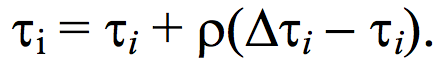
\includegraphics[width=3cm,keepaspectratio]{images/phero_update.png}
\end{figure}

onde $\rho$ é a taxa de evaporação do feromônio e $\Delta\tau_i$ é taxa de atualização do feromônio, calculada a cada iteração como:

\begin{figure}[H]	
  \centering
  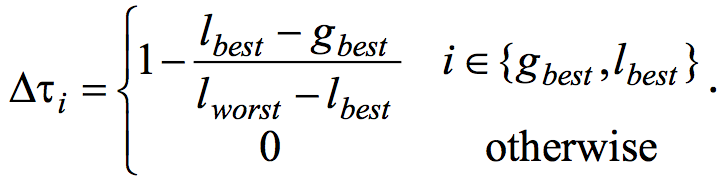
\includegraphics[width=6cm,keepaspectratio]{images/delta_t.png}
\end{figure}

onde $g_best$, $l_best$ e $l_worst$ são os valores totais das distâncias entre os nós na melhor solução global, melhor solução local e pior solução local, respectivamente. Como consequência dessa fórmula mantemos os feromônios nos thresholds setados anteriormente. 

Assim que atualizados os feromônios, a melhor solução global pode ser atualizada, caso seja esse o caso.

\subsection{Controle de estagnação} \label{sub:stagnation}

Como consequência do MMAS, é possível que após certo número de iterações o sistema estagne em suas soluções, com $p$ nós apresentando feromônio igual a $\tau_{max}$, e os restantes $n - p$ nós apresentando feromônios iguais a $\tau_{max}$. A estagnação pode ser detectada com a equação:

\begin{figure}[H]	
  \centering
  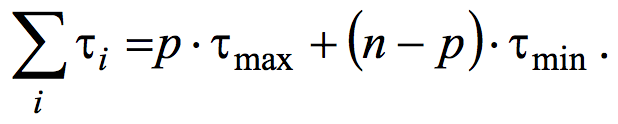
\includegraphics[width=4.5cm,keepaspectratio]{images/stagnation.png}
\end{figure}

Caso os dois lados da equação sejam iguais, os feromônios são resetados para o valor inicial, no entanto mantendo a melhor solução global armazenada.

\subsection{Otimização do código}
Python não é nem de longe a melhor linguagem de programação para se implementar problemas de otimização e de aprendizado de máquina, pois estes são problemas que exigem muito processamento. Processamento é o principal problema enfrentado por Python, por abstrair muitos dos detalhes computacionais, além de ser interpretada ao invés de compilada. 

Para que a execução dos experimentos se desse de forma mais rápida então a biblioteca \texttt{NumPy}, cuja utilização se dá em C, foi amplamente utilizada, com a maioria das operações iterativas tendo sido adaptadas para cálculos com matrizes. A biblioteca \texttt{Cython} também foi utilizada em 3 dos módulos criar para gerar diretamente código C, assim também agilizando o processo de execução. Com todas essas mudanças o código passou a rodar 2.5 vezes mais rápido no total.

Para que o código Cython(extensão .pyx) possa ser executado juntamente com o código em Python(extensão .py) é necessário antes executar o script auxiliar \texttt{setup.py} da seguinte forma:

\begin{center}
\begin{verbatim}
    python3 setup.py build_ext --inplace
\end{verbatim}
\end{center}

